\chapter{Literature Review}
\label{chap:lr}

This chapter is a representative review of recent works most directly related to the thesis problem statement. It is not intended as a systematic review of the full swarm-security literature; instead, it synthesizes a focused corpus covering swarm communication, lightweight cryptography, decentralized trust, and adaptive security.

\section{Communication Architectures of Swarm Systems}
\label{sec:swarm_comm_arch}

Swarm robotics is grounded in self-organization, local interaction, and emergent collective behavior. Surveys by Dias et al.~\cite{diasSwarmRoboticsPerspective2021} and Debie et al.~\cite{debieSwarmRoboticsSurvey2023} show that scalability and fault tolerance are central advantages of swarm systems, but they also make reliable communication a critical dependency.

Varadharajan et al.~\cite{varadharajanSwarmRelaysDistributed2020} addressed connectivity in dynamic environments through the \textit{Swarm Relays} algorithm, which builds distributed self-healing communication chains across heterogeneous robots. Arseneault et al.~\cite{arseneaultRASSRiskAwareSwarm2022} proposed \textit{RASS}, a risk-aware storage framework that distributes replicas according to environmental hazard. Together, these studies show that decentralized coordination and survivability can be achieved without centralized infrastructure, but they leave confidentiality and authentication only partially addressed.

Swarm network topologies vary from mesh to cluster-based configurations in order to manage connectivity and scalability. Mesh topologies provide path redundancy and self-recovery under node failures; star structures centralize information flow, simplifying key management at the cost of a single point of failure; cluster-based organization balances local autonomy with hierarchical coordination, reducing communication overhead.

Topology selection influences attack resilience: mesh networks resist selective interception but require complex key management; star systems are vulnerable to compromise of the central node; cluster-based architectures localize damage but require secure inter-cluster communication channels.

Self-healing communication chains maintain continuous network coverage under dynamic changes. Robots autonomously reconfigure links by detecting disruptions and establishing alternative routes. Risk-aware storage and routing approaches further improve resilience by placing critical data away from high-risk regions of the swarm~\cite{arseneaultRASSRiskAwareSwarm2022}.

These approaches establish an important foundation for robust swarm networking, yet they do not by themselves provide a complete secure communication stack. Encryption, authentication, and adaptive key management are still required to protect the information exchanged over these resilient topologies, as summarized in Table~\ref{tab:comm_arch_comparison}.

\begin{table}[H]
\centering
\caption{Comparison of communication architectures of swarm systems}
\label{tab:comm_arch_comparison}
\scriptsize
\renewcommand{\arraystretch}{1.14}
\begin{tabularx}{\textwidth}{|p{2.2cm}|p{2.4cm}|p{2.0cm}|X|p{2.5cm}|}
\hline
\textbf{Architecture} & \textbf{Topology} & \textbf{Fault Tolerance} & \textbf{Security Integration} & \textbf{Application} \\
\hline
Swarm Relays & Hybrid mesh-chain & High & Connectivity oriented, no built-in encryption & Ground--air heterogeneous swarms \\
\hline
RASS & Cluster-based & Medium & Risk awareness without message confidentiality & Distributed data storage \\
\hline
Mesh topology & Fully connected & High & Requires complex key management & Large-scale UAV swarms \\
\hline
Star topology & Centralized & Low & Simplified, single point of failure & Small specialized groups \\
\hline
Cluster-based & Hierarchical & Medium & Inter-cluster protection required & Multi-level heterogeneous systems \\
\hline
\end{tabularx}
\end{table}

This comparison highlights a recurring design tension: the architectural choices that improve robustness often complicate secure message exchange. That tension motivates lightweight, decentralized cryptographic mechanisms that can operate within the same resource envelope as the swarm itself.

\section{Lightweight Cryptography}
\label{sec:lightweight_crypto}

Lightweight cryptography for constrained agents has been extensively studied. Han et al.~\cite{hanLightweightSecureCommunication2025} show that elliptic-curve methods remain attractive for UAV swarms because they reduce key size and communication overhead relative to conventional PKI while still supporting authenticated key establishment.

Symmetric authenticated encryption provides the practical data-plane counterpart to asymmetric setup. AES-GCM is efficient when hardware support is available, whereas ChaCha20-Poly1305 is often better suited to software-only microcontrollers~\cite{nistFips197AES,nistSP80038DGCM,rfc8439}. These schemes offer confidentiality and integrity with low per-message cost once a shared secret has been established.

Token-based and proof-based mechanisms further reduce runtime overhead. Ferrer et al.~\cite{ferrerSecureSecretCooperation2021} demonstrate how cryptographic proofs can support secure cooperation without exposing raw mission data. Manikandan and Sriramulu~\cite{manikandanASMTPAnonymousSecureMessaging2024} develop ASMTP, a token-based protocol for UAV swarms that combines lightweight authentication with anonymity preservation. Broader IoT authentication and lightweight-hash surveys show the same pressure toward compact authenticators and hardware-aware hash design~\cite{kumarComprehensiveSurveyAuthenticationIoT2022,sakanLightweightHashFunction2025,khanSurveyLightweightHardwareHash2025}. These approaches show that security can be made compatible with constrained communication loops, but they typically remain static once deployed.

The main limitation of these methods is not the absence of efficient primitives, but the absence of adaptive control. Fixed cryptographic configurations are easy to reason about, yet they waste resources in low-risk phases and may be insufficient during high-risk phases. An adaptive framework is therefore attractive because it can preserve lightweight operation by default while escalating protection when the mission context changes.

\begin{figure}[H]
\centering
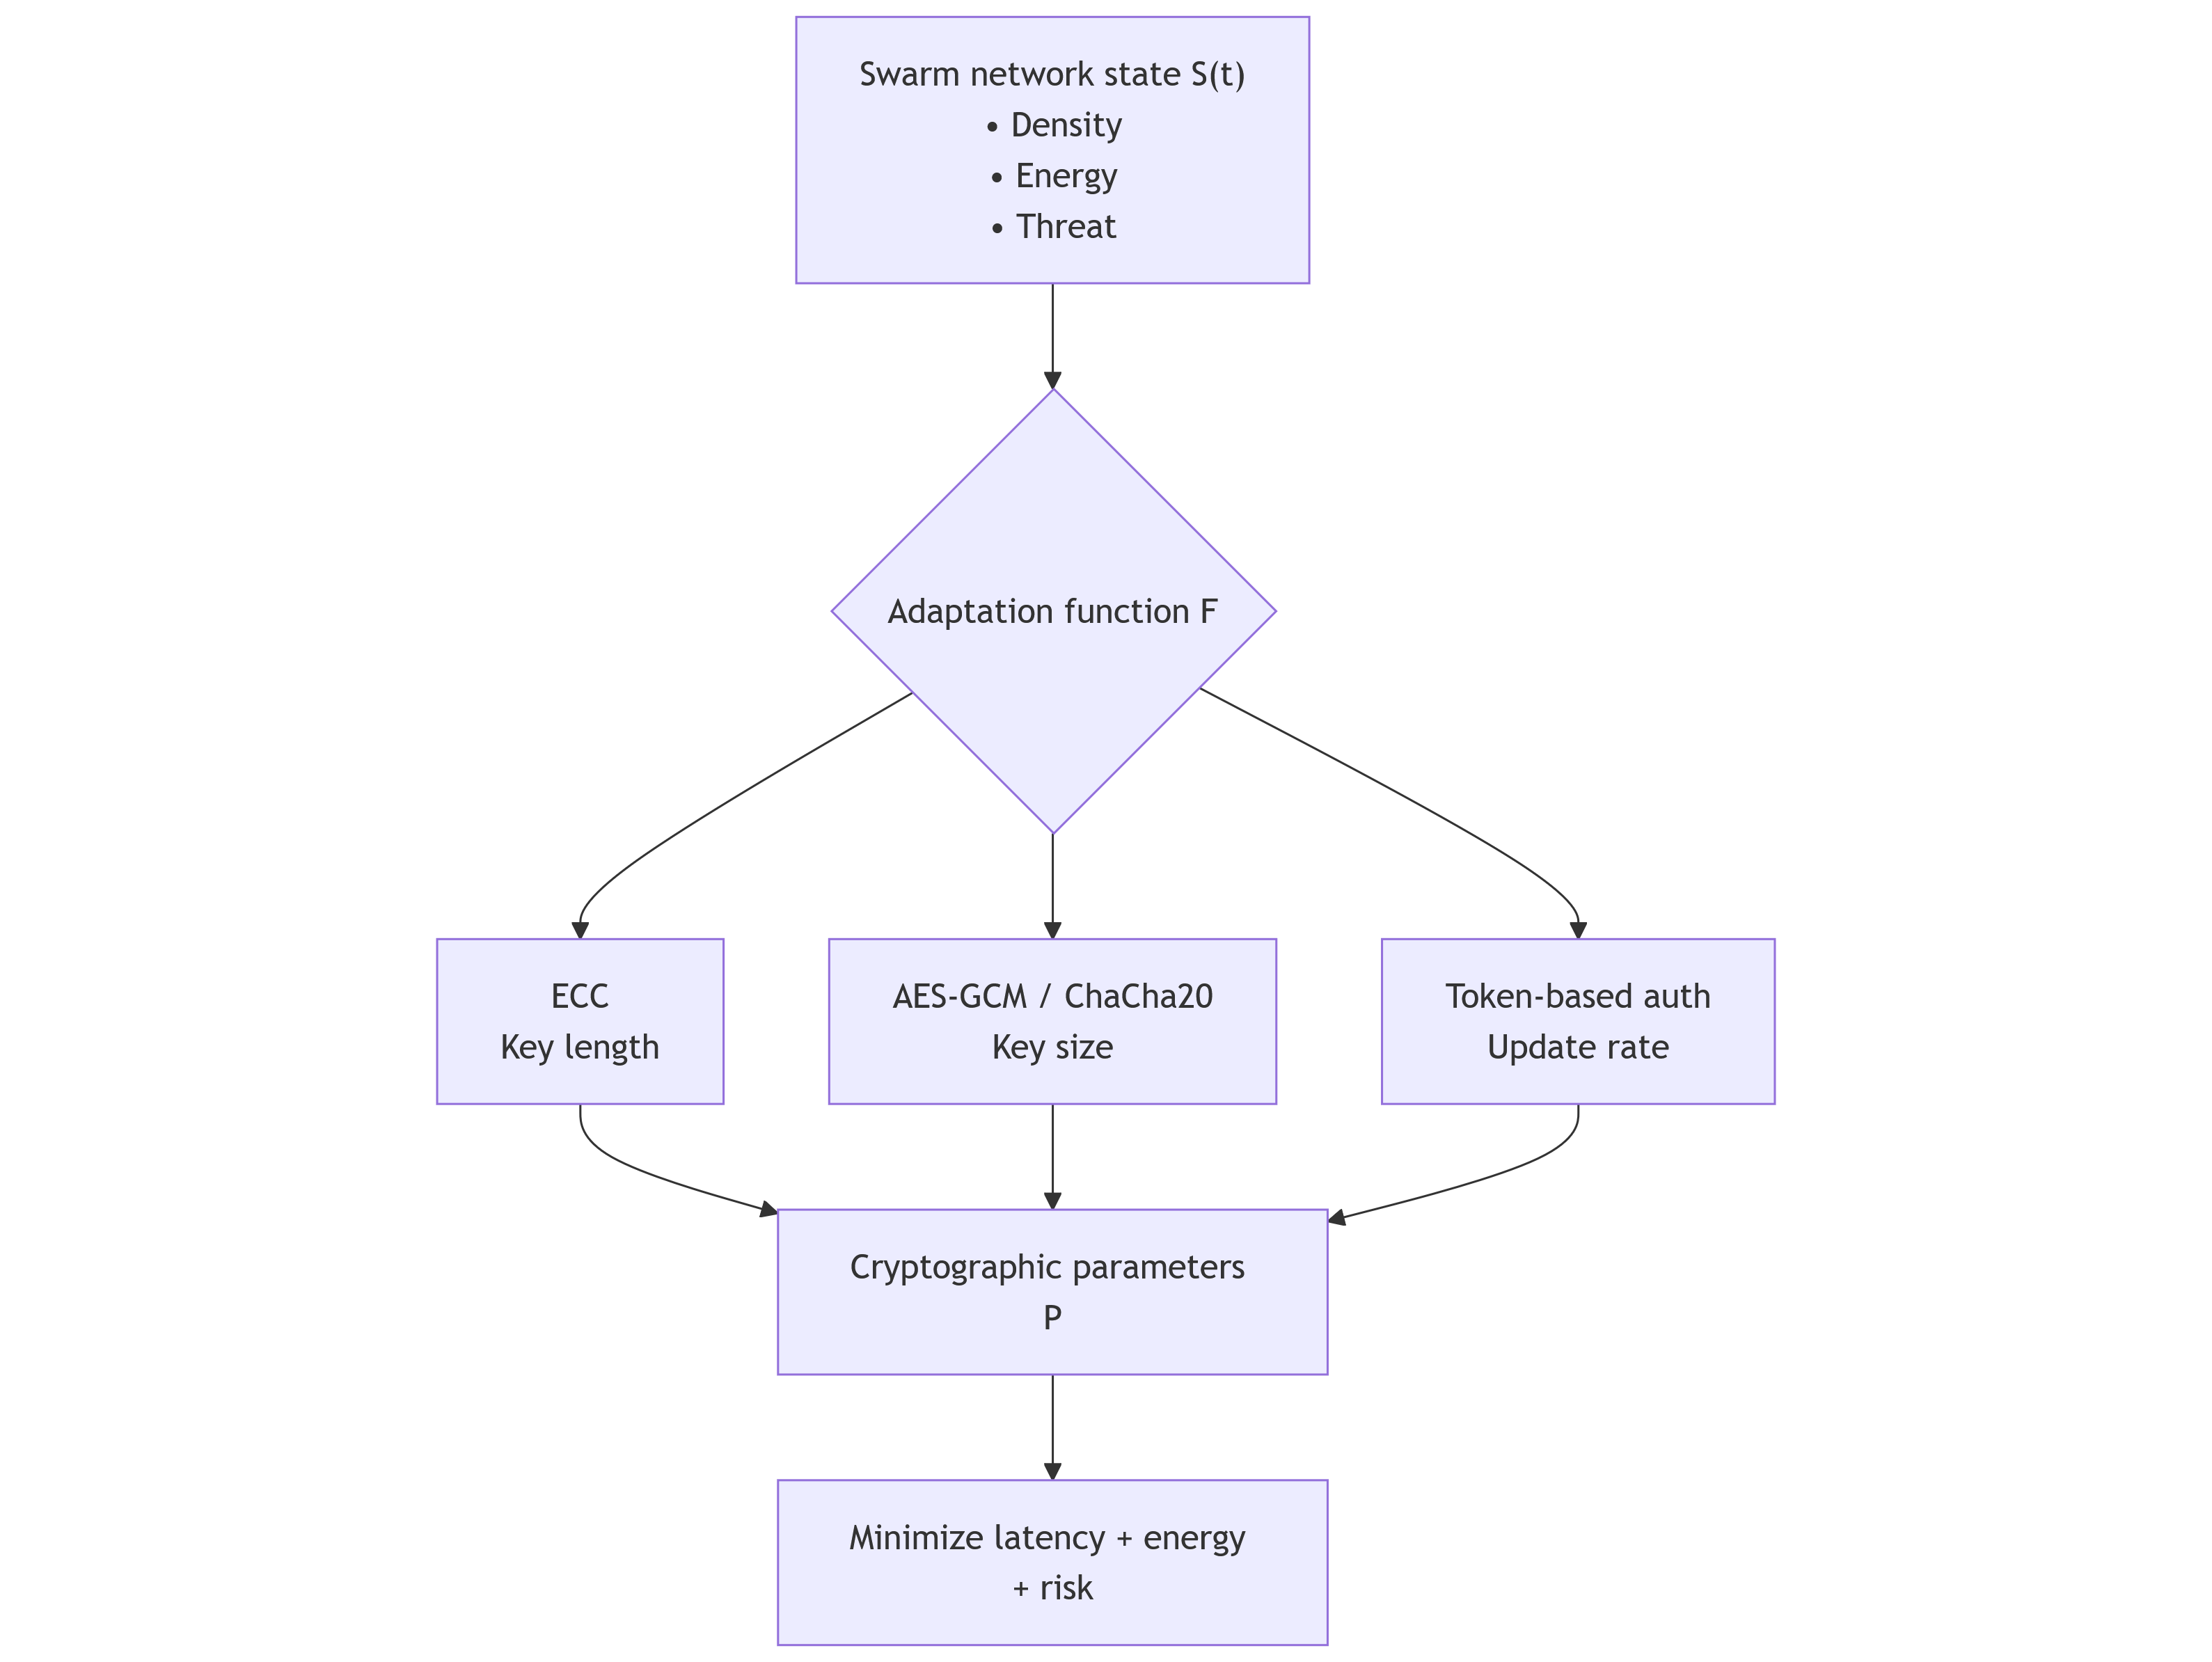
\includegraphics[width=0.9\textwidth]{figs/adaptive_crypto_framework}
\caption{Conceptual model of adaptive cryptographic selection based on swarm state.}
\label{fig:adaptive_crypto}
\end{figure}

Figure~\ref{fig:adaptive_crypto} summarizes this idea: observed swarm state is mapped to a cryptographic configuration that balances latency, energy use, and security level instead of fixing one operating mode for the entire mission.

\section{Decentralized Trust Mechanisms}
\label{sec:decentralized_trust}

To eliminate single points of failure, several studies extend swarm security with blockchain or distributed trust mechanisms. Sun and Shao~\cite{sunResearchDataSecurityEmergency2022} propose a blockchain-based communication scheme for heterogeneous emergency-response swarms, while Pacheco et al.~\cite{pachecoSecuringFederatedLearning2024} use blockchain to secure federated learning in robot swarms. Related trustless-agreement work similarly explores how robot collectives can provide distributed evidence for external decisions~\cite{pachecoSwarmOracleTrustless2025}. These works emphasize auditability and tamper resistance, but they also indicate a heavier protocol stack than the lightweight data-plane mechanisms discussed in the previous section.

Kohli et al.~\cite{kohliSwarmNetFirmwareAttestation2024} address trust from a different angle with \textit{Swarm-Net}, a firmware-attestation framework for IoT swarms based on graph neural networks and volatile-memory fingerprints. Adjacent adversarial-IoT and swarm-malware detection work reinforces the need to treat endpoint trust and runtime anomaly detection as separate but complementary layers~\cite{bommanaAddressingAdversarialAttacks2025,hanifOrchestratingMLSwarmMalware2025}. This work is relevant because it focuses on node integrity rather than message protection, illustrating that secure swarm systems require both trustworthy endpoints and secure channels.

Collectively, these studies reveal a persistent trade-off. Stronger decentralized trust mechanisms improve system assurance, but they are often too heavy for fast control loops or resource-constrained agents. Lightweight cryptographic approaches scale better, but they do not by themselves provide collective agreement or system-wide attestation.

\section{Adaptive Security Frameworks}
\label{sec:adaptive_security}

The reviewed literature suggests that secure swarm communication must combine three properties: lightweight runtime protection, decentralized operation, and adaptation to mission context. Existing works typically emphasize only one or two of these properties at a time. Connectivity-oriented designs prioritize resilience, lightweight schemes prioritize efficiency, and blockchain-style approaches prioritize trust.

Context-dependent security has been explored in adjacent IoT settings. Phalaagae et al.~\cite{phalaagaeEnergyEfficientAuthenticationCluster2024} show in clustered wireless sensor environments that authentication choices can be tuned to deployment constraints. Energy-aware encryption and zero-energy IoT discussions point in the same direction: protection mechanisms must be selected with the device power envelope in mind~\cite{khashanSmartEnergyEfficientEncryption2024,abbasTowardsZeroenergyNavigating2024}. In this thesis, that work is used as an adjacent-domain motivation for adaptive security rather than as direct swarm-robotics evidence.

For swarm robotics, this motivates an adaptive framework in which network density, remaining energy, packet loss, and threat estimates influence the choice of key length, cipher, authentication mode, and key-rotation policy. Such a framework does not replace the underlying primitives; instead, it orchestrates them according to mission state.

\section{Gap Analysis}
\label{sec:gap_analysis}

Within the reviewed corpus, three practical gaps remain most relevant to the present thesis. \textit{Static protocol configuration}: many lightweight schemes are evaluated with fixed security parameters even though mission conditions vary over time. \textit{Fragmented security layers}: communication resilience, trust, and message protection are often analyzed separately. \textit{Limited executable comparison}: adaptive ideas are frequently motivated conceptually, but common benchmark comparisons between stronger static, lighter static, and adaptive profiles are still rare in the selected literature.

These observations justify a narrower thesis contribution: an adaptive lightweight framework with retained formal reasoning and an executable benchmark for pairwise operating-mode comparison. They do not, by themselves, establish that the proposed benchmark is a complete swarm-security evaluation; that limitation is addressed explicitly in the later chapters.
